% Created 2024-12-22 Sun 18:36
% Intended LaTeX compiler: pdflatex
\documentclass[10pt]{article}
% =================================BASE====================================%
\usepackage[left=2cm,right=2cm,top=2cm,bottom=2cm]{geometry} % Marges
\usepackage[T1]{fontenc} % Nécessaire avec FrenchBabel
\usepackage[utf8]{inputenc} % Important pour symboles Francophones, é,à,etc
\usepackage{csquotes} % Recommandé par PDFLatex lors de la compilation. 

% Calligraphie
%\usepackage{pxfonts} % Met le texte ET les maths en Palatino + donne accès à des symboles math
%\usepackage{palatino} % Cette commande met seulement le texte en police palatino
\usepackage{lmodern} % Pour les maths? Lmodern pour les maths
\usepackage{cfr-lm} % Use lmodern for sans-serif
\usepackage{mathrsfs} % Permet la command \mathscr (Lettres attachées genre) \mathscr(ABC)
\usepackage{eucal}   % Vient changer le \mathcal{ABC} parce que celui de base est laid.

% Bibliographie
\usepackage[backend=biber,sorting=ynt,maxbibnames=99,style=authoryear]{biblatex}
\addbibresource{master-bibliography.bib}

% Stuff
\usepackage{amsmath, amssymb, amsthm} % Symb. math. (Mathmode+Textmode) + Beaux théorèmes.
\usepackage{mathtools,cancel,xfrac} % Utilisation de boîtes \boxed{} + \cancelto{}{}, xfrac
\usepackage{graphicx, wrapfig} % Géstion des figures.
\usepackage{hyperref} % Permettre l'utilisation d'hyperliens.
\usepackage{color} % Permettre l'utilisation des couleurs.
\usepackage{colortbl} % Color tables
\usepackage[dvipsnames]{xcolor} % Couleurs avancées.

% Physique
\usepackage{physics} % Meilleur package pour physicien. 

% Style
\usepackage{pgf,tikz} % Realisation de figures TIKZ.
\usetikzlibrary{arrows.meta,bending, shapes.geometric, automata, positioning, decorations.pathreplacing, math} % Arrow heads et les formes de noeuds
\usepackage{empheq} % Boite autour de MULTIPLE équations
\usepackage{bbding}

% Français
\usepackage[french]{babel} % Environnements en Français.
\frenchbsetup{
StandardLists=true,
StandardItemLabels=true} % Sinon, french modifie les itemize
\usepackage{titling} % Donne accès à \theauthor, \thetitle, \thedate
% ==============================BASE-(END)=================================%





% ================================SETTINGS=================================%
% Pas d'indentation en début de paragraphe :
\setlength\parindent{0pt}
\setlength{\parskip}{0.15cm}

% Tableaux/tabular
% Espace vertical dans les tabular/tableaux
\renewcommand{\arraystretch}{1.2}

% Couleurs de hyperliens :
\definecolor{mypink}{RGB}{147, 0, 255}
\hypersetup{colorlinks, 
             filecolor=mypink,
             urlcolor=mypink, 
             citecolor=mypink, 
             linkcolor=mypink, 
             anchorcolor=mypink}
\definecolor{color1}{RGB}{148,220,236}
\definecolor{color2}{RGB}{84,76,163}
\definecolor{color3}{RGB}{108,156,227}
\definecolor{color4}{RGB}{244,164,156}
\definecolor{color5}{RGB}{252,204,164}


% Numéros d'équations suivent les sections :
\numberwithin{equation}{section} 


% Les « captions » sont en italique et largeur limitée
\usepackage[textfont = it]{caption} 
\captionsetup[wrapfigure]{margin=0.5cm}


% Retirer l'écriture en gras dans la table des matières
\usepackage{tocloft}
\renewcommand{\cftsecfont}{\normalfont}
\renewcommand{\cftsecpagefont}{\normalfont}


% MODIFICATION DES TITLESECS et SUBTITLESEC
% On a des lignes à droite des sections et sous-sections
\usepackage[explicit]{titlesec}
    % Raised Rule Command:
    % Arg 1 (Optional) - How high to raise the rule
    % Arg 2 - Thickness of the rule
    \newcommand{\raisedrulefill}[2][0ex]{\leaders\hbox{\rule[#1]{1pt}{#2}}\hfill}
    \titleformat{\section}{\Large\bfseries}{\thesection. }{0em}{#1\;\raisedrulefill[0.4ex]{0.25pt}}
    \titleformat{\subsection}{\large\bfseries}{\thesubsection. }{0em}{#1\;\raisedrulefill[0.4ex]{0.10pt}}


% MODIFICATION DES LISTES : 
\renewcommand{\labelitemi  }{{\raisebox{0.35\height}{\tiny$\blacksquare$}}}
\renewcommand{\labelitemii }{{\raisebox{0.35\height}{\tiny$\blacktriangleright$}}}
\renewcommand{\labelitemiii}{$\bullet$}

\renewcommand{\boxtimes}{\blacksquare}
% ================================SETTINGS=================================%



% ==============================NEWCOMMANDS================================%
% CQFD symbol
\renewcommand{\qedsymbol}{$\hfill\blacksquare$}
\newcommand{\cqfd}{\hfill$\blacktriangleleft$}

% Vecteurs de base :
\newcommand{\nvf}{\vb{\hat{n}}}
\newcommand{\evf}{\vb{\hat{e}}}
\newcommand{\ivf}{\vb{\hat{i}}}
\newcommand{\jvf}{\vb{\hat{j}}}
\newcommand{\kvf}{\vb{\hat{k}}}
\newcommand{\uu}{\vb{u}}
\newcommand{\vv}{\vb{v}}
\newcommand{\ust}{\vb{u}_{\ast}}
\newcommand{\xx}{\vb{x}}
\newcommand{\rad}{\text{Rad}}

% Physics empty spaces 
\newcommand{\short}{\vphantom{pA}}
\newcommand{\tall}{\vphantom{pA^{x^x}_p}}
\newcommand{\grande}{\vphantom{\frac{1}{xx}}}
\newcommand{\venti}{\vphantom{\sum_x^x}}
\newcommand{\pt}{\hspace{1pt}} % One horizontal pt space

% Moyenne numérique entre deux points de grilles. 
\newcommand{\xmean}[1]{\overline{#1}^x}
\newcommand{\ymean}[1]{\overline{#1}^y}
\newcommand{\zmean}[1]{\overline{#1}^z}
\newcommand{\xymean}[1]{\overline{#1}^{xy}}

% Tilde over psi
\newcommand{\tpsi}{\tilde{\psi}}
\newcommand{\tphi}{\tilde{\phi}}

% Nota Bene env :
%\newcommand{\nb}{$\boxed{\text{\footnotesize\EightStarConvex}\pt \mathfrak{N. B.}}$\hspace{4pt}}
\newcommand{\nb}{\underline{{\footnotesize\EightStarConvex}\pt $\mathfrak{N.B.}$\vphantom{p}}\hspace{3pt}}

% Opérateur de transformée de Fourier. 
\newcommand{\fourier}{\operatorname{\raisebox{-0.4em}{\resizebox{2em}{!}{$\mathscr{F}$}}}}

% Mettre (a,b) à la suite d'une série d'équations horizontales.
\newcommand{\ab}{\refstepcounter{equation}\tag{\theequation a,b}}
% ==============================NEWCOMMANDS================================%



% ==============================PAGE-TITRE=================================%
% Titlepage 
\newcommand{\mytitlepage}{
\begin{titlepage}
\begin{center}
{\Huge \thesubtitle \par}
\vspace{2cm}
{\Huge \MakeUppercase{\thetitle} \par}
\vspace{2cm}
RÉALISÉ DANS LE CADRE\\ D'UN PROJET POUR \par
\vspace{2cm}
{\Huge ISMER--UQAR \par}
\vspace{2cm}
{\thedate}
\end{center}
\vfill
Rédaction \\
{\theauthor}\\
\url{charles-edouard.lizotte@uqar.ca}\\
ISMER-UQAR\\
Police d'écriture : \textbf{CMU Serif Roman}
\end{titlepage}
}
% ==============================PAGE-TITRE=================================%



% =================================ENTÊTE==================================%
\usepackage{fancyhdr}
\pagestyle{fancy}
\setlength{\headheight}{13pt}
\renewcommand{\headrulewidth}{0.0pt} % Ligne horizontale en haut

\fancyhead[R]{\underline{\textit{Section \thesubsection}}}
\fancyhead[L]{\underline{\textit{\thepage}}}
\fancyfoot[R]{\textit{\theauthor}}
\fancyfoot[L]{}
\fancyfoot[C]{} 
% =================================ENTÊTE==================================%
\author{Charles-Édouard Lizotte}
\date{15/11/2024}
\title{Rapport hebdomadaire}
\newcommand{\thesubtitle}{Contrat Été 2024}
\hypersetup{
 pdfauthor={Charles-Édouard Lizotte},
 pdftitle={Rapport hebdomadaire},
 pdfkeywords={},
 pdfsubject={},
 pdfcreator={Emacs 29.4 (Org mode 9.7.11)}, 
 pdflang={French}}
\begin{document}

\mytitlepage
\tableofcontents\newpage
\section{Switches de glace et le modèle}
\label{sec:org5d88e57}

\subsection{Mise en contexte}
\label{sec:orga5903e4}

\textit{<2024-11-11 Mon> } Où en sommes-nous aujourd'hui? Le modèle est capable d'assimiler tous les fichiers d'input de ma configuration. Par contre, la routine du modèle \emph{ww3 shel} est incapable d'assimiler certains fichiers de glace, comme le diamètre moyen des floes dans une case \(\expval{D}\).\bigskip

Essentiellement, la routine \emph{ww3 shel} prend 4 fichiers d'input, soit
\begin{itemize}
\item \textbf{Ice param. 1} : La \emph{ice thickness}.
\item \textbf{Ice param. 5} : Le \emph{mean ice diameter}.
\item \textbf{Wind} : Le vent.
\item \textbf{Ice field} : La concentration de glace.
\end{itemize}

J'ai pris les \emph{switches} que Jeremy m'avait données. Donc,la \emph{switch} de glace, c'est \textbf{IC4}, par contre je n'ai pas pris letemps de définir une \emph{Ice method} dans la routine \emph{ww3 grid}. La \emph{switch} IC4 propose six méthodes différentes. Je vais prendre celle qui ressemble le plus à la maîtrise d'Eliot Bismuth, soit le \emph{scaling} polynomial de \Textcite{kohout2008elastic}.\bigskip

Donc, est-ce que ça vient des \emph{switches} ou est-ce que mes fichiers d'input sont mal construits? Je pense que ça vient des \emph{switches}, c'est pourquoi, je refais la mise à niveau que Dany voulait, juste ici. \medskip

\textit{<2024-11-13 Wed> } Il a malheureusement été prouvé que mon problème venait de mes \emph{inputs}, plutôt que des \emph{switches}\ldots{}
\subsection{Remise en contexte sur les switches}
\label{sec:org5d0b280}

Selon la documentation de Wavewatch \autocite[p.16]{wwiii2016user}, tous les termes sont \emph{scalés} par la concentration de glace \(f_i\). Lorsqu'on lance la routine d'assimilation de la grille \emph{ww3 grid}, on obtient

\begin{quote}
\textbf{Dissipation via ice parameters (SIC4).}

\emph{Sice will be calculated using Empirical method.}

\emph{Required field input: ice parameters (varies).}

\emph{\&SIC4}

\emph{IC4METHOD=1          ,}

\emph{IC4KI= 10*0.00000000      ,}

\emph{IC4FC= 10*0.00000000      ,}
\end{quote}

Donc, c'est très peu d'information. Selon la documentation, il nous faut quand même l'épaisseur de la glace. Pourtant, selon la documentation \autocite{wwiii2016user}, 
\subsection{Switch IC4}
\label{sec:org083d0ab}

Dans la version que Jeremy m'avait donnée, il utilisait la \emph{switch} IC4. Selon la documentation,

\begin{quote}
\emph{Frequency-dependent damping by sea ice.}
\end{quote}

Voyons ce que cette \emph{switch} nous demande en terme d'inputs, parce le modèle ne semble pas avoir besoin du \emph{ice parameter 5}, soit le diamètre moyen des floes (\emph{ice diameter}). En fait, ça tombe sous le sens, parce qu'il n'y a aucune mention de la taille des floes dans la documentation, même si initialement ça venait de l'article de \Textcite{kohout2008elastic}, il me semble. \medskip

Selon la documentation, la méthode \emph{frequency dependent} semble venir de C. Collins et E. Rogers (Faudrait vérifier cette info). Il faut mettre un ICE4METHOD dans la \emph{namelist} de la routine \emph{ww3 grid}. Les méthodes 1 à 6 existent.
\begin{itemize}
\item 1) an exponential fit to the field data of Wadhams et al. (1988),
\item 2) the polynomial fit in Meylan et al. (2014),
\item 3) a quadratic fit to the calculations of Kohout and Meylan (2008) given in Horvat and Tziperman (2015),
\item 4) Eq. 1 of Kohout et al. (2014) qui reprend les polynomes de \Textcite{kohout2008elastic}.
\item 5) a simple step function with up to 4 steps (maybe nonstationary and non-uniform), and
\item 6) a simple step function with up to 10 steps (must be stationary and uniform).
\end{itemize}

Concrètement, nous avons pris la \textbf{méthode 3}, car c'est celle qu'Eliot Bismuth avait empruntée.
\subsection{Inputs}
\label{sec:org6dc9c79}

\textit{<2024-11-05 Tue> } Je crois que j'ai trouvé la source du problème. Tout viendrait peut-être de la convention océanographique. Si c'est le cas, je trouve ça génant. Selon la documentation du module \emph{wavespectra},

\begin{quote}
\emph{Wave direction coordinate in coming-from convention, with name dir, defined in (required for 2D spectra and directional methods).}
\end{quote}

Donc il va falloir réévaluer les directions : la routine \emph{ww3 shell} nous permet de définir des champs homogènes -- comme le vent par exemple -- avec une direction. Aussi, la routine \emph{ww3 strt} nous permet de définir un spectre directionnel \(E(f,\theta)\), de JONSWAP ou Pierson-Moskowitz en utilisant la convention océanographique. Par contre, dans cette sous-routine, on nous mentionne explicitement que \(270^\circ\) représente l'ouest. Reste à savoir si on définit nos quantités en amont ou en aval de l'écoulement.\bigskip

\begin{figure}[!h]
\begin{center}
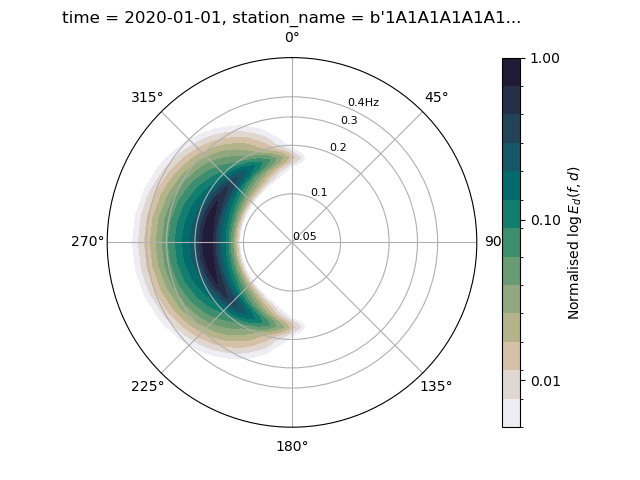
\includegraphics[width=0.7\textwidth]{Figures/figures/jonswap-wavespectra3.png}
\begin{minipage}{0.7\textwidth}
\caption{Spectre de JONSWAP orienté à 270 degré (convention océanographique). Concrètement, ça signifit que les vagues proviennent de l"ouest et se propagent à l'est.}
\label{fig:jonswap}
\end{minipage}
\end{center}
\end{figure}


\textit{<2024-11-13 Wed> } Après mure inspection, si je construit un fichier NetCDF dans lequel le vent s'écoule en x-y vers l'est, j'obtiens des \emph{output} de directions moyennes des vagues \(\expval{\theta}\) de \(270^\circ\). Donc, on a notre réponse, je crois. On définit la provenance des vagues et non la direction de propagation moyenne des vagues c'est ce qui explique tous les problèmes que j'ai eu jusqu'à maintenant.
\subsubsection{Grille du modèle}
\label{sec:org0c3fa5d}

Toutes les quantités importantes pour la création de la grille de notre simulation sont compilées dans le tableau \ref{tab:orgd0ec2a1}. 

\begin{table}[!h]
\caption{\label{tab:orgd0ec2a1}Quantités importantes en ce qui a trait à la grille de Wavewatch III.}
\centering
\begin{tabular}{lcrcl}
\hline
\hline
Description & Symbole & Valeur & Unités & Note\\
\hline
\emph{Freq. Increment Factor} & \(IF\) & 1.07 & -- & \autocite[Voir][switch NL2]{wwiii2016user}\\
Fréquence initiale & \(f_{min}\) & 0.05 & \(\mathrm{s}^{-1}\) & Suggéré dans la maîtrise de Bismuth.\\
Fréquences maximale & \(f_{max}\) & 0.749 & \(\mathrm{s}^{-1}\) & \(f_{max} = f_{min}\cdot(IF)^{nf}\)\\
Nombre de fréquences & \(nf\) & 40 & -- & \autocite[Voir][switch NL2]{wwiii2016user}\\
Nombre de directions & \(n_\theta\) & 36 & -- & \autocite[Voir][switch NL2]{wwiii2016user}\\
Pas de temps & \(\Delta t\) & 20.00 & s & \(\Delta t < \Delta x/c^{max}_g\)\\
\hline
Taille de la grille & \(L_x\) & 5 & km & Point de grille d'un GCM.\\
Taille des points de grille & \(\Delta x\) & 500 & m & 10 divisions.\\
Nombre de points en x & \(n_x\) & 10 & -- & Petit domaine.\\
Nombre de points en y & \(n_x\) & 3 & -- & Petit domaine.\\
points de mer & \(n_{sea}\) & 8 & -- & Voir figure \ref{org511b3c8}\\
Profondeur du domaine & \(L_z\) & 200 & m & Pas très profond.\\
\hline
\end{tabular}
\end{table}

Concrètement, la grille de fonction ou la \emph{mapsta} devrait ressembler à la figure \ref{org511b3c8}. 


\begin{figure}
\begin{center}
\begin{tikzpicture}
   \fill [ForestGreen!10] (0,0) rectangle (10,3);
   \fill [blue!15] (1,1) rectangle (9,2);
   \fill [white] (0,1) rectangle (1,2);
   \fill [white] (9,1) rectangle (10,2);
   \fill [red!15] (1,1) rectangle (2,2);
   \draw[dotted] (0,0) grid (10,3);
   \draw[thick] (0,0) rectangle (10,3);
%%%
   \draw[|{latex}-{latex}|] (10.25,0) -- (10.25,3);
   \draw (10.25,1.5) node [rotate=90,below] {$150$ m};
   \draw[|{latex}-{latex}|] (0,-0.25) -- (10,-0.25);
   \draw (5,-0.5) node [below] {$500$ m};
%%%
   \filldraw [dotted] (-0.25,0.5) -- (0.5,0.5);
   \filldraw [dotted] (-0.25,2.5) -- (0.5,2.5) circle (1pt);
   \draw [decoration={brace}, decorate, thick] (-0.25,0.5) -- (-0.25,2.5);
   \draw (-0.5,1.5) node [rotate=90,above] { 25m à 125m};
%%%
   \filldraw [dotted] (0.5,3.25) -- (0.5,2.5);
   \filldraw [dotted] (9.5,3.25) -- (9.5,2.5) circle (1pt);
   \draw [decoration={brace}, decorate, thick] (0.5,3.25) -- (9.5,3.25);
   \draw (5,3.5) node [above] { 25m à 475m};
 %%%
   \filldraw (0.5,0.5) circle (1pt);
   \draw (0.5,0.5) node [right] {(25m,25m)};
\end{tikzpicture}
\end{center}
\caption{\label{org511b3c8}MAPSTA ou grille de fonction de Wavewatch III.}
\end{figure}


On remaque qu'on s'éloigne des bords, parce que ce n'est pas très clair ce que le modèle fait sur les bords. 
\subsubsection{Conditions frontières (Boundary points)}
\label{sec:org6bdb22c}


\begin{table}[htbp]
\caption{\label{tab:org106a1e3}Paramètres du spectre de vagues assimilié comme conditions frontière à l'ouest du domaine.}
\centering
\begin{tabular}{lcrcl}
\hline
\hline
Description & Symbole & Valeur & Unités & Notes\\
\hline
Constante pour Goda & -- & 0.205 & ? & \Textcite{goda1988variablity}\\
\emph{Energy level of PM spectrum} & \(\alpha\) & 0.0081 & -- & \Textcite{wwiii2016user} (Constante de Phillips)\\
\emph{Peak enhancement factor} & \(\gamma\) & 3.3 & -- & \Textcite{hasselmann1973measurements,wwiii2016user}\\
\emph{Spread with GAMMA} & \(\sigma_A\) & 0.07 & -- & \Textcite{hasselmann1973measurements,wwiii2016user}\\
\emph{Spread with GAMMA} & \(\sigma_B\) & 0.09 & -- & \Textcite{hasselmann1973measurements,wwiii2016user}\\
Moyenne directionnelle & \(\theta_m\) & 90 & degrés & \Textcite{wwiii2016user} (Convention océanographique)\\
\hline
\emph{Peak frequency} & \(f_m\) & 1/6 & Hz & (Maîtrise d'Eliot Bismuth)\\
Hauteur significative des vagues & \(h_s\) & 1 & m & (Maîtrise d'Eliot Bismuth)\\
\hline
\end{tabular}
\end{table}


Selon la \href{https://wavespectra.readthedocs.io/en/latest/construction.html\#jonswap}{documentation du module Wavespectra}, l'équation pour le spectre JONSWAP \autocite{hasselmann1973measurements} est codée de sorte à ce que 
\begin{equation}
   S(f) = \alpha g^2 (2\pi)^{-4} f^{-5} \exp{-\frac{5}{4} \left (\frac{f}{f_p} \right)^{-4} } \gamma^{\exp{\frac{(f-f_p)^2}{2\sigma^2f_p^2}}},
\end{equation}
soit dépendant de la hauteur des vagues. Toujours selon la documentation de Wavespectra, si la hauteur significative des vagues est fournie, alors le spectre de JONSWAP est normalisé de sorte à ce que \(4\sqrt{m_0} = Hs\), sinon le spectre est normalisé par \(\alpha\) comme dans l'équation précédente.
Puis l'étalement directionnel est donné par
\begin{equation}
   G(\theta,f)=F(s)cos^2\qty[\frac{1}{2}(\theta-\theta_{m})],
\end{equation}
où \(F(s)\) est seulement un paramètre de normalisation. Le résultat, c'est la figure \ref{fig:jonswap}.
\subsubsection{Présence de glace}
\label{sec:org51856c3}

Pas grand chose à dire ici, a part que les champs ont les valeurs mentionnées dans le tableau \ref{tab:org535f41d}.

\begin{table}[!h]
\caption{\label{tab:org535f41d}Tableau tiré de la maîtrise d'Éliot Bimuth.}
\centering
\begin{tabular}{lcrc}
\hline
\hline
Description de la variable & Symbole & Valeur & Unités\\
\hline
Épaisseur des floes & \(h\) & 0.5 & m\\
Diamètre moyen des floes & \(\expval{D}\) & 200 & m\\
Hauteur significative des vagues & \(H_s\) & 1 & m\\
\hline
\end{tabular}
\end{table}
\subsection{Gestion de la « spectral tail »}
\label{sec:orgdaf86cf}

Nous y sommes! Enfin, la \emph{spectral tail} commence à nous faire des siennes. Regardons de plus près nos \emph{switches} :

\begin{itemize}
\item On emprunte la méthode NL1, donc l'utilisation des DIA, comme dans la méthode de Sébastien Dugas. Déjà, nous ne devrions pas tant avoir de problème de \emph{spectral tail}. Il semble qu'une partie du spectre soit non-définit lorsque le vent est trop fort, comme nous avions dans le cas du modèle Julia.
\end{itemize}

Avec des vents de moyenne amplitude, ça ne semble pas être le cas dutout. Peut-être que la méthode des DIA est à revoir pour de fort vents. Mentionnons qu'à la formation de la grille, le modèle nous signale que

\begin{quote}
\emph{Triad interactions not defined.}
\end{quote}

ce qui veut dire que les triades ne sont tout simplement pas définies. Pourtant, les DIA sont super bien définies :

\begin{quote}
\textbf{Nonlinear interactions (DIA) (default values) :}\\
    \emph{Lambda                      :    0.25}\\
    \emph{Prop. constant              : 0.278E+08}\\
    \emph{kd conversion factor        :    0.75}\\
    \emph{minimum kd                  :    0.50}\\
    \emph{shallow water constants     :    5.50  0.83 -1.25}
\end{quote}
\subsection{Problèmes de génération de vagues?}
\label{sec:orga2ab524}

\textit{<2024-11-18 Mon> } Même lorsqu'il n'y a pas de vent -- donc aucune génération de vagues -- il y a des vagues qui s'accumulent sur la partie est de notre config. Pourtant, à l'extrémité est de notre config, il n'y a pas de frontière, c'est seulement un « point ouvert ». Voici quelques pistes de solution. 

\begin{itemize}
\item \textbf{Est-ce que le modèle voit des murs? Si oui, quel est l'effet du coefficient de réflexion. Essayons de l'enlever dans un cas sans glace et aucun vent.} Aucune différence. Il semble que les vagues s'accumulent toujours à l'est. Ce n'est pas ce que nous devrions voir. Plutôt, on devrait voir c'est un motif ressemblant à ce qu'on retrouve à l'ouest. Du moins, on devrait voir un spectre décroissant à l'inverse de ce qu'on a ici.

\item \textbf{Malgré le fait que notre point sur le bord est un point ouvert, j'ai l'impression que le modèle voit ce point là comme une frontière physique, ce qui pourrait expliquer l'accumulation de vagues dans ce coin là.} Après avoir testé, nous sommes dans la même situation. Les vagues s'accumulent dans l'extrémité est de notre domaine sans aucune raison. Ce sont des vagues avec une plus grande période, ce qui pourrait nous donner l'impression que ça vient de notre spectre initial, mais avec un trasfert d'énergie progressif.

\item \textbf{Est-ce que c'est vraiment du à une réflexion? Testons avec beaucoup plus de points pour voir}. On a le même problème. Même que le problème semble de plus en plus fort. J'ai aussi testé avec une frontière physique et aucune réflexion, le résultat est le même. Donc, il faudrait commencer à vérifier les \emph{switches} probablement.

\item \textbf{Réessayons sans aucun \emph{input} à la frontière ouest, donc les vagues sont nulles. On revient à 12 points de long, avec réflexions, puis on enlève le point frontière.} Le problème ne semble plus exister. Ce que j'en déduis, c'est qu'une partie de l'énergie sert à créer de petites vagues qui vont croître en se déplaçant vers l'est. C'est bizarre, car il n'y a pas de vent qui causerait la création de vages.

\item \textbf{Enlevons la switch de réflexion}. Même problème! Ce n'est donc \textbf{pas un problème de réflexion}.

\item \textbf{Mettons des conditions frontière bien plus intenses pour voir}. Ça ne change rien.
\end{itemize}
\subsection{Dénouement du problème}
\label{sec:orgb6ec42f}

\begin{itemize}
\item Le problème n'est pas causé par les réflexions;
\item Le problème n'est pas causé par la présence de points non-définit à l'extrémité est;
\item Bien que le fait de retirer les conditions frontières à l'ouest semble éliminer le problème.
\end{itemize}

\textbf{Solution :} J'ai réussi, il semble. C'était un problème de pas de temps et de longueur e domaine. Lorsqu'on mettait un très long domaine, on obtenait des oscillations bizarres dans le spectre vers l'extrémité « est ». Pourtant, je croyais que ma condition CFL était bonne.

\begin{itemize}
\item Maintenant, il n'a pas d'lair de se passer grand chose, mais on est de retour avec le problème de la \emph{spectral tail}.
\end{itemize}

\printbibliography
\end{document}
